%%Berichtvorlage für EDBV WS 2015/2016

\documentclass[deutsch]{scrartcl}
\usepackage[top=1cm,left=1cm,right=1cm,bottom=1cm]{geometry}
\usepackage[ngerman]{babel}
\usepackage[utf8]{inputenc}
\usepackage{algorithmic}
\usepackage{algorithm}
\usepackage{graphicx}
\usepackage{amsmath,amssymb}
\usepackage{subcaption}
\captionsetup{compatibility=false}
\usepackage{multirow}
\usepackage{color}

\begin{document}

\title{Lib-Indexer} %%Projekttitel hier eintragen

%%Namen und Matrikelnummern der Gruppenmitglieder hier eintragen
\author{Anand Eichner, Laurenz E. Fiala, Anna Nieto-Berezhinskaya, Aleksandar Vucenovic}
\date{\vspace{-5ex}}



%%------------------------------------------------------

\maketitle

\begin{figure}[h!]
	
	\centering
	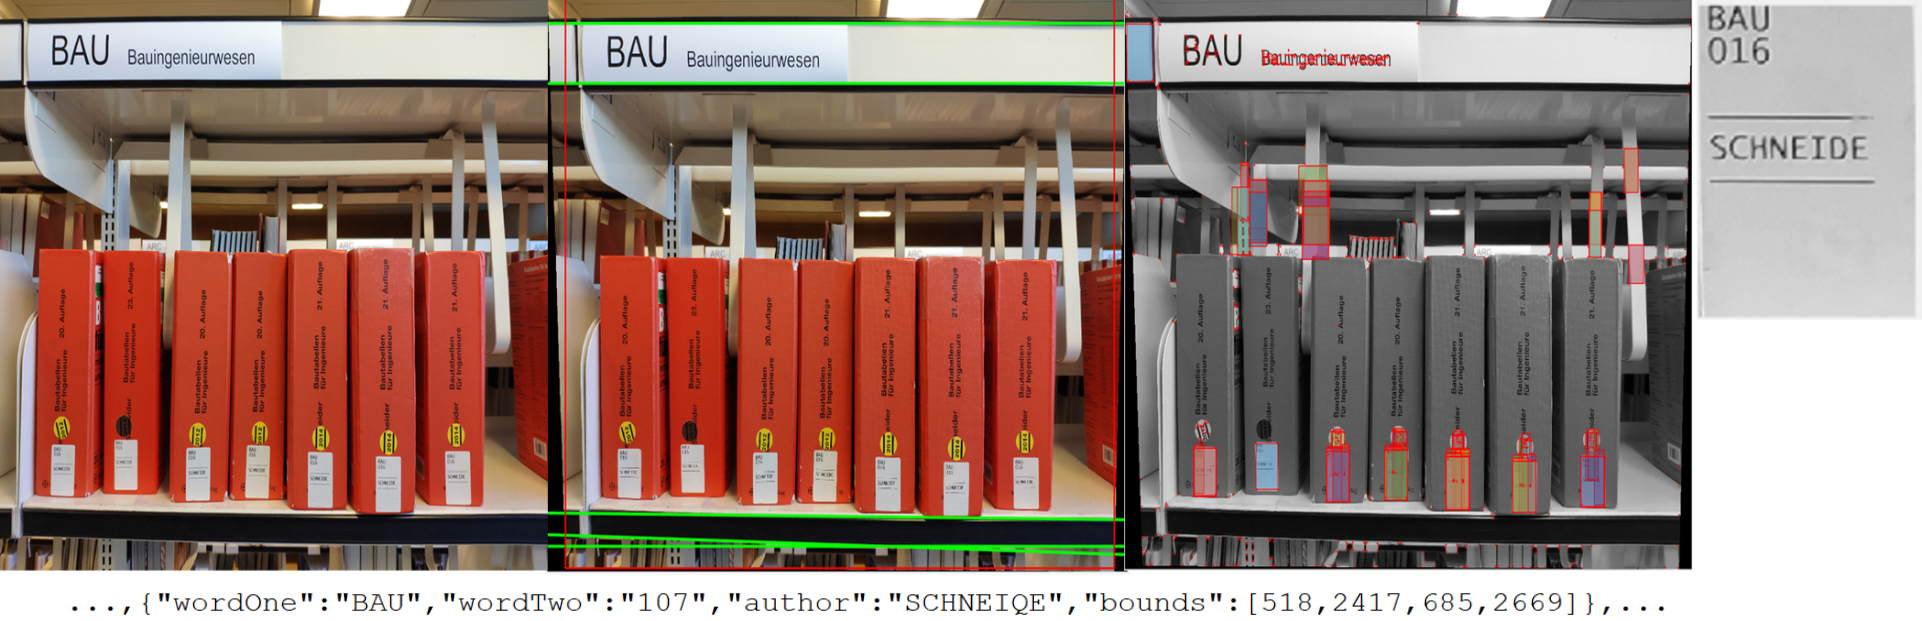
\includegraphics[width=0.8\textwidth]{poster.png}
	\caption{Lib-Indexer-Pipeline}
	\label{fig:erg}
\end{figure}

%%------------------------------------------------------

\section*{Projekt}
Der Lib-Indexer soll aus einem Bild eines Bücherregels der TU Wien, Bücher erkennen und den Inhalt der Etiketten als strukturiereten Text ausgeben.

\section*{Vorgangsweise}

Beschreibung der Pipeline

\begin{enumerate}
	\item Ein Bild eines Bücherregals der TU-Bibliothek wird eingelesen
	\item Mittels einer Hough-Transformation und einer geometrischen Verzerrung wird die Perspektive des Bildes korrigiert. Nach diesem Schritt sind die Regalfächer horizontal im Bild.
	\item Ein Otsu-Threshold wird genutzt, um die Labels vom Bildhintergund abzugrenzen.
	\item Ein Harris-Eckendetektor erkennt die Ecken der Buchetiketten.
	\item Mit dem relativen Abstand zwischen den Regalfächern wird ein Akzeptanzbereich für die Dimensionen der Etiketten  erstellt.
	\item Integral Imaging wird genutzt, um den Label-Hintergrund mit dem Text zu Vergleichen. Wenn das Verhältnis im Akzeptanzbereich liegt, wird das Label an die OCR weitergereicht.
	\item Optical Character Recognition wird genutzt, um die Schrift auf den Etiketten vom Bild in Textform umzuwandeln (Es werden zwei Arten unterstützt: Sum of Squared Differences und Normalized Cross-Correlation).
\end{enumerate}

\section*{Ergebnisse}
Ergebnis in Abbildung~\ref{fig:erg}.




\end{document}
